\documentclass{article} 
\usepackage{tikz} 
\usetikzlibrary{positioning, arrows}
\usepackage[a4paper]{geometry}
\begin{document}
 
% Project A: Lifelines
% Visualise the relationships within the Edwardses and the Jonga family.
% Use a digital pinboard such as TaskCards or Canva to create a visual lifeline.
% Document their journey, conflicts, lows and highs chapter by chapter. Briefly outline what happens in each chapter.
  
\section*{Relationships}
\begin{center} 
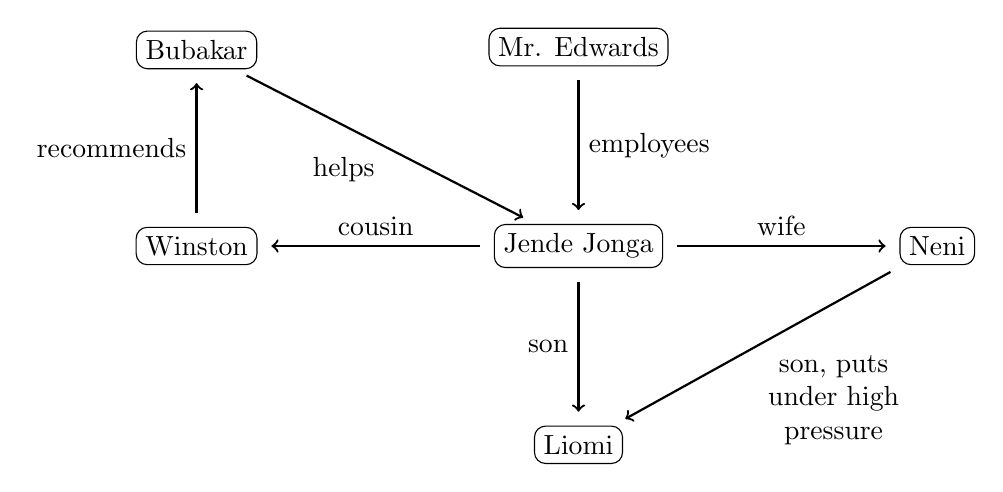
\begin{tikzpicture}[
    node distance=2cm and 3cm,
    every node/.style={draw, rectangle, rounded corners, align=center, minimum width=0.5cm},
    every edge/.style={draw, thick, ->, shorten >=5pt, shorten <=5pt}
]
\node (jende) {Jende Jonga};
\node (neni) [right=of jende] {Neni}; 
\node (liomi) [below=of jende] {Liomi}; 
\node (winston) [left=of jende] {Winston}; 
\node (bubakar) [above=of winston] {Bubakar}; 
\node (edwards) [above=of jende] {Mr. Edwards};
 
\path
 (jende) edge [above] node[fill=none, draw=none] {wife} (neni)
 (jende) edge [left] node[fill=none, draw=none] {son} (liomi)
 (neni) edge [below right] node[fill=none, draw=none] {son, puts \\ under high \\ pressure} (liomi)
 (jende) edge [above] node[fill=none, draw=none] {cousin} (winston)
 (winston) edge [left] node[fill=none, draw=none] {recommends} (bubakar)
 (bubakar) edge [below left] node[fill=none, draw=none] {helps} (jende)
 (edwards) edge [right] node[fill=none, draw=none] {employees} (jende);
\end{tikzpicture}
\end{center} 
 
\section*{Lifeline}
\begin{center} 
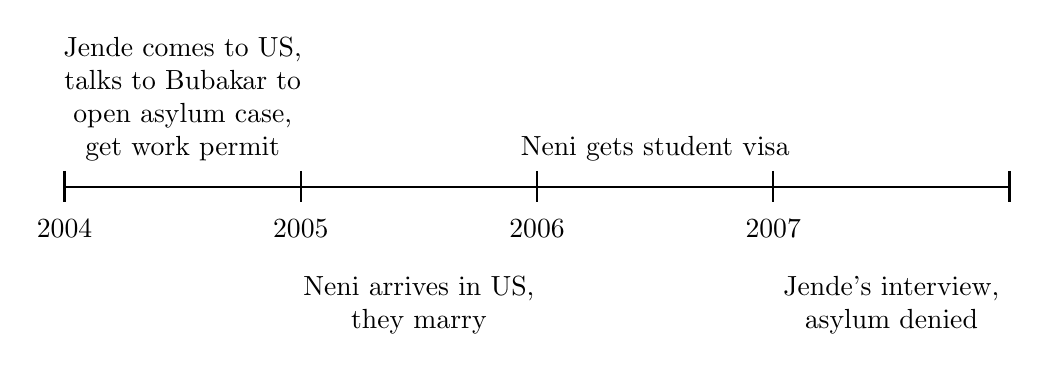
\begin{tikzpicture}
 \draw[thick, -] (0,0) -- (12,0);
 \foreach \x/\year in {0/2004, 3/2005, 6/2006, 9/2007} {
  \draw[thick] (\x,0.2) -- (\x,-0.2);
  \node[below] at (\x, -0.3) {\year};
 }
 \draw[thick] (12,0.2) -- (12,-0.2);
 
 \node[above, align=center] at (0.5 * 3, 0.2) {Jende comes to US, \\ talks to Bubakar to \\ open asylum case, \\ get work permit};
 \node[above, align=center] at (1.5 * 3, -2) {Neni arrives in US, \\ they marry};
 \node[above, align=center] at (2.5 * 3, 0.2) {Neni gets student visa};
 \node[above, align=center] at (3.5 * 3, -2) {Jende's interview, \\ asylum denied};
\end{tikzpicture}
\end{center} 
 
\section*{Outlines} 
\begin{description}
 \item[Chapter 1] It's 2007. Jende, who is in America with his wife Neni and their son Liomi, has a job interview.
 \item[Chapter 2] Neni and Fatou talk a bit while shopping in Chinatown.
 \item[Chapter 3] Jende gets hired as Mr. Edward's chauffeur, which everyone is happy about. His cousin, Winston, recommends an immigration lawyer, Bubakar, to him to help him fight for his asylum.
 \item[Chapter 4] Jende is exhausted but happy after his first day at his new job, Neni's school is going well and she's making plans of becoming a pharmacist. They're both hopeful for the future, planning for a better life in a bigger apartment.
 \item[Chapter 5] While Jende is driving, Vince Edward says that he won't come to Aspen, leading to a conflict between Clark and Cindy.
 \item[Chapter 6] Jende talks exclusively positively about his hometown, Limbe, but also explains that he moved to America to live the American Dream.
 \item[Chapter 7] Jende talks to Leah, Clark's secretary, for the first time. She's nice to Jende but at the same time also kinda talks down on him. They discuss work, Leah says that its not going too well for the company. 
 \item[Chapter 8] Neni has to work hard, do lots of chores, help Liomi, learn for school, e.\,t.\,c. 
 \item[Chapter 9] Terrible events unfold, like that one time Jende's father was deadly sick with malaria: Bubakar calls him to say that his Asylum case was denied, but that they'll continue fighting for it. He and Neni can't cope with it at all.
 \item[Chapter 10] Neni notices signs of pregnancy, but has to go to teachers conference quickly. Liomi's teacher explains that he's doing pretty well at school, just that he gets distracted by the class clown Billy sometimes. Neni scolds Liomi for this and puts a lot of pressure on him, saying that he has to be good at school and get a high paying job. She herself gets a B- in her Precalculus class, which she isn't happy with.
\end{description} 
 
 
\end{document}
 
 
 
 
